\documentclass[UTF8]{ctexart}
\ctexset{
  section={
    format=\raggedright\zihao{3},
    name={T,}
  },
  subsection={
    format={\zihao{4}},
    number={\arabic{subsection}}
  }
}
\usepackage[a4paper,left=3cm,right=3cm,top=2cm]{geometry}
\usepackage{amsmath}
\usepackage{enumitem}
\usepackage{float}
\usepackage{threeparttable}
\usepackage{caption}
\usepackage{multirow}
\usepackage{graphicx}
\usepackage{listings}
\usepackage{color}
\renewcommand{\figurename}{Figure}
\definecolor{dkgreen}{rgb}{0,0.6,0}
\definecolor{gray}{rgb}{0.5,0.5,0.5}
\definecolor{mauve}{rgb}{0.58,0,0.82}
\lstset{frame=tb,
  language=C,
  aboveskip=3mm,
  belowskip=3mm,
  showstringspaces=false,
  columns=flexible,
  basicstyle={\small\ttfamily},
  numbers=left,%设置行号位置none不显示行号
  %numberstyle=\tiny\courier, %设置行号大小
  numberstyle=\color{gray},
  keywordstyle=\color{blue},
  commentstyle=\color{dkgreen},
  stringstyle=\color{mauve},
  breaklines=true,
  breakatwhitespace=true,
  escapeinside=`,%逃逸字符(1左面的键),用于显示中文例如在代码中`中文...`
  tabsize=4,
  extendedchars=false %解决代码跨页时,章节标题,页眉等汉字不显示的问题
}

\setlength\lineskiplimit{5.25bp}
\setlength\lineskip{5.25bp}

\title{ICS Homework 1}
\author{崔士强 PB22151743}
\date{\today}

\bibliographystyle{plain}

\begin{document}

\maketitle
\section{}
\subsection{}
$-114_{ten}=1000\ 1110_{two}$

$+81_{ten}=0101\ 0001_{two}$
\subsection{}
$0011\ 0010_{two}=50_{ten}$

$1111\ 1101_{two}=-3_{ten}$
\section{}
\subsection{}
smallest: $-128_{ten}$

largest: $127_{ten}$
\subsection{}
range: $-2^N$ to $2^N-1$
\section{}
$-64_{ten}$
\section{}
\subsection{}
While the value of $a-b$ exceeds the largest value of the data type int.
\subsection{}
Then the program will give the right answer. That's because under the rules of 2's complement, when a - opeator
is put before a, the computer will invert all bits of a and add 1. That gives $2^N-a$ in unsigned int representation.
\section{}
$4098\frac{1}{256}$
\section{}
smallest number: $1\ 11111111\ 11111111111111111111111$

smallest positive number: $0\ 00000000\ 00000000000000000000000$
\section{}
0 
\section{}
\subsection{}
\begin{lstlisting}
  void swap(int *a, int *b){
    *c= *a ^ *b;
    *a= *a ^ *c;
    *b= *b ^ *c;
  }
\end{lstlisting}
\subsection{}
\clearpage
\section{}
\begin{figure}[h]
  \centering
  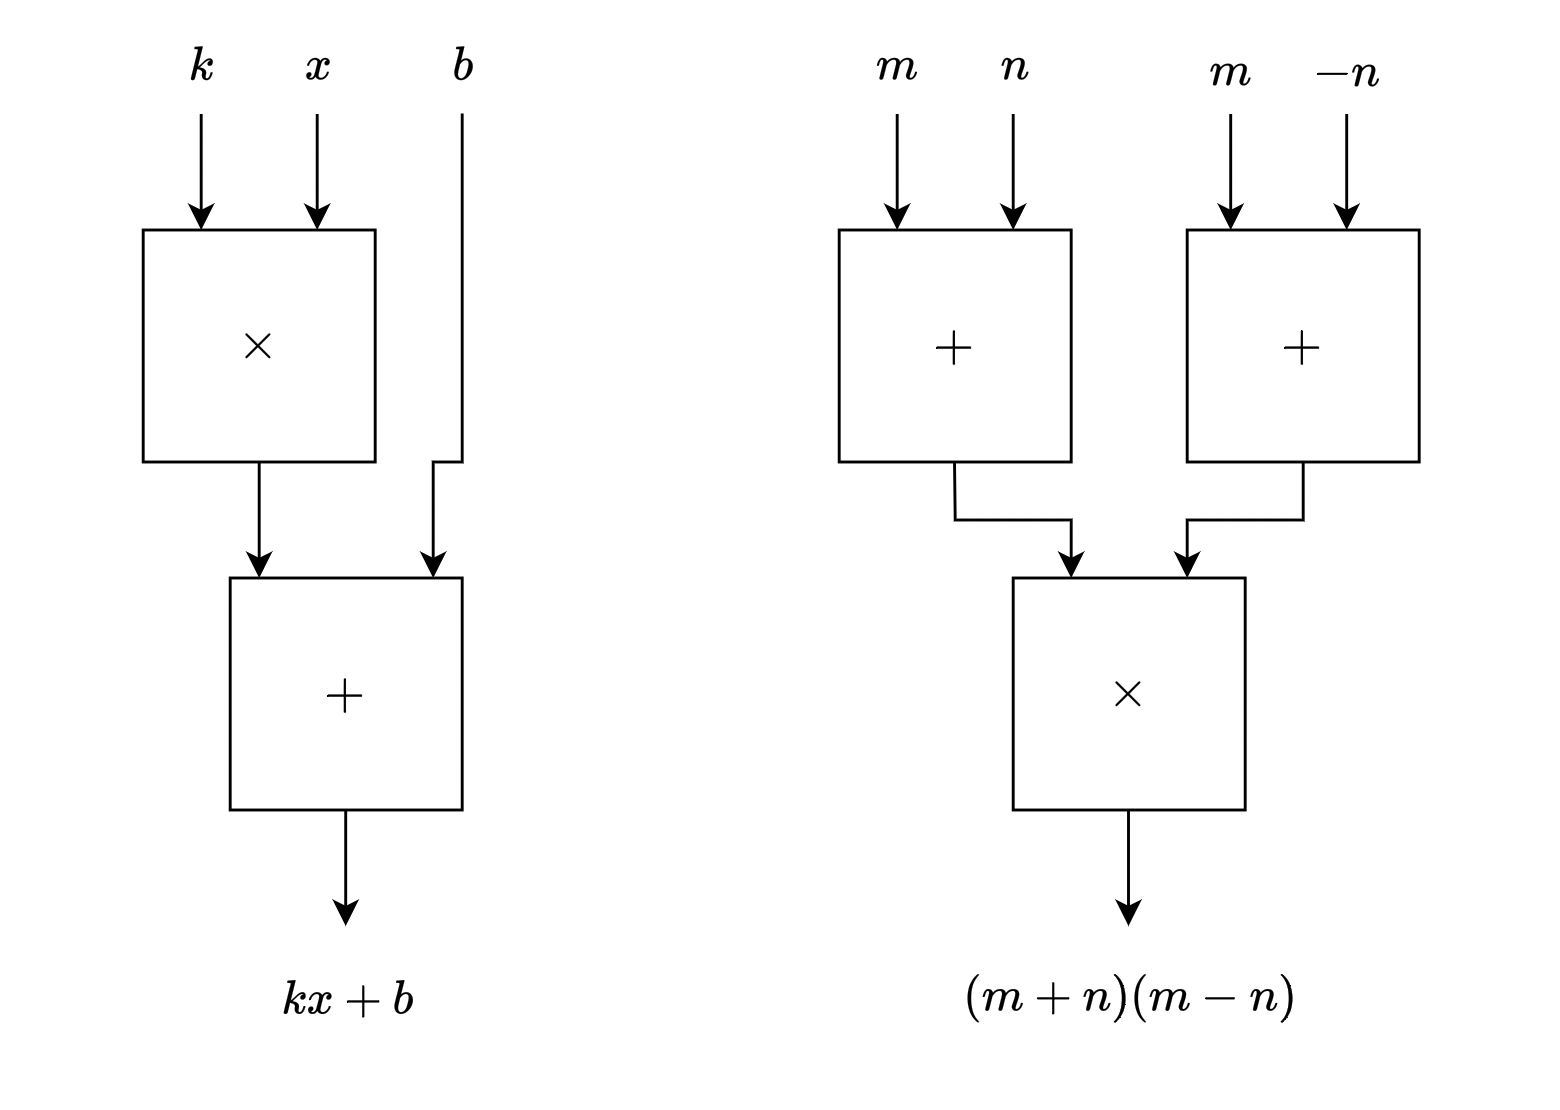
\includegraphics[scale=0.3]{hw_1.png}
  \caption{9.1\&9.2}
\end{figure}
\begin{figure}[h]
  \centering
  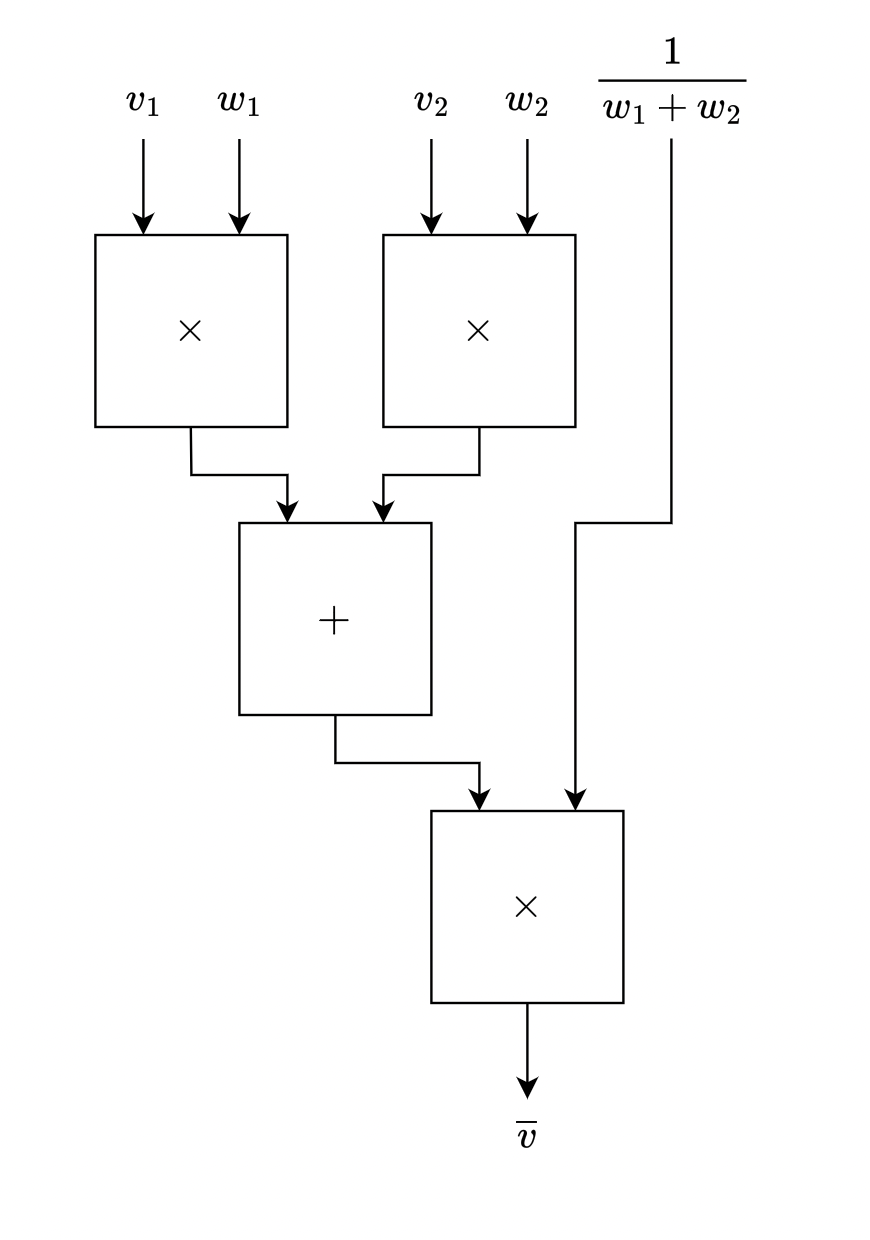
\includegraphics[scale=0.3]{hw_1_2.png}
  \caption{9.4}
\end{figure}
\section{}
\subsection{}
$2^6=64$

So we need 6 bits.
\subsection{}
$6N$
\subsection{}
$000111\ 011101\ 100101\ 100101\ 101000\ 111111\ 010110\ 101000\ 101011\ 100101\ 011101\ 111110$


\bibliography{math}

\end{document}
\iffalse
\begin{figure}[h]
    \centering
    \includegraphics[scale=0.5]{name.png}
    \caption{name}
\end{figure}
\fi
